\documentclass[review]{elsarticle}
\usepackage[utf8]{inputenc} 
\usepackage{lineno,hyperref}
\usepackage{tabu}
\usepackage{float}
\usepackage{tabularx}
\usepackage{subfigure}
\usepackage[fleqn]{amsmath}
\modulolinenumbers[5]

\journal{Journal of Applied Thermal Engineering}

%%%%%%%%%%%%%%%%%%%%%%%
%% Elsevier bibliography styles
%%%%%%%%%%%%%%%%%%%%%%%
%% To change the style, put a % in front of the second line of the current style and
%% remove the % from the second line of the style you would like to use.
%%%%%%%%%%%%%%%%%%%%%%%

%% Numbered
%\bibliographystyle{model1-num-names}

%% Numbered without titles
%\bibliographystyle{model1a-num-names}

%% Harvard
%\bibliographystyle{model2-names.bst}\biboptions{authoryear}

%% Vancouver numbered
%\usepackage{numcompress}\bibliographystyle{model3-num-names}

%% Vancouver name/year
%\usepackage{numcompress}\bibliographystyle{model4-names}\biboptions{authoryear}

%% APA style
%\bibliographystyle{model5-names}\biboptions{authoryear}

%% AMA style
%\usepackage{numcompress}\bibliographystyle{model6-num-names}

%% `Elsevier LaTeX' style
\bibliographystyle{elsarticle-num}
%%%%%%%%%%%%%%%%%%%%%%%

\begin{document}

\begin{frontmatter}

\title{Low load operating protocol investigation of a 620MWe power boiler using an indirectly coupled process model}

%% Group authors per affiliation:
\author{B.T. Rawlins}
\author{R. Laubscher\corref{mycorrespondingauthor}}
\cortext[mycorrespondingauthor]{Corresponding author}
\ead{ryno.laubscher@uct.ac.za}
\author{P. Rousseau}
\address{Department of Mechanical Engineering, Applied Thermal-Fluid Process Modeling Research Unit, University of Cape Town, Library Rd, Rondebosch, Cape Town, 7701, South Africa}

\begin{abstract}

Low load operation of utility boiler

\end{abstract}

\begin{keyword}
CFD\sep Eulerian-Eulerian\sep Boiler \sep Low-load operation
\end{keyword}

\end{frontmatter}

\linenumbers

\begin{center}
\begin{tabular}{|p{0.075\textwidth}p{0.3\textwidth}p{0.05\textwidth}p{0.075\textwidth}p{0.3\textwidth}p{0.05\textwidth}|} 
 \hline
\multicolumn{3}{|l}{\textbf{Nomenclature}} & &  &\\
\textit{Symbol} & \textit{Quantity} & \textit{Unit} & & &\\
$A$ &  Area & $m^2$ & & &\\
$A_p$ & Particle surface area & $m^2$& & & \\
$d_p$&Particle diameter & $m$ & & & \\
$E$& Fluid total energy&$J/kg$ & & & \\
$E_a$& Reaction activation energy&$J/kmol$ & & & \\
$P$& Pressure & $Pa$ & & & \\
$T_g$& Gas temperature& $K$ & & & \\
$T_p$&Particle temperature & $K$& & & \\
$u$& Velocity &$m/s^2$ & & &\\
\hline
\end{tabular}
\end{center}

\section{Introduction}
The use of coal fired power plants (CFPP) to provide electricity generation is intended to be phased out in order to mitigate the ingress of climate change. However, the switch to more sustainable generation sources pose great challenges for developing countries due to the long transition times and costs involved \cite{ugum2019}. Due to the abundance of coal resource present in South Africa CFPPs are the dominant power generation source, with approximately 80 $\%$ of the energy needs being met using CFPPs \cite{eskom}. The promising integration of renewable energy and the decommissioning of old CFPPs in South Africa, will push CFPP from a primarily base load operation to a mid-merit/flexible operating protocol. This will inherently mean CFPPs will need to operate at low-loads for continuous time periods. 

Mathematical models that can accurately capture the behaviour of the boilers thermal-hydraulic response at varying loads can be used to determine the safe and efficient operating limits \cite{Laubscher2019b}. Since, the long term deviation from design conditions can lead to operational incapabilities affecting combustion stability \cite{Hernik2020}, an increase in harmful emissions \cite{Chang2021} and the localised overheating of heat exchangers due to insufficient cooling being provided by the internal working fluid \cite{Modlinski2019}.

The full scale testing or experimentation of CFPPs is deemed to expensive to pursue, thus the use of computational fluid dynamics (CFD) allows for the modelling of a full-scale CFPPs, at steady-state, to be investigated at various loads circumnavigating the use of time-consuming and costly field tests. CFD simulations have been successfully used to model a variety of CFPP boiler types (\cite{Laubscher2019a}, \cite{Gu2020}) and cover various aspects such as pollution control (\cite{Du2017},\cite{Fan2001}), gas-solid flow effects (\cite{Chen2017}) and boiler retrofitting (\citep{Gu2020}, \cite{He2007}).

Recent CFD studies investigating low-load operation of CFPP boilers have focused on the combustion stability, harmful emissions and the gas flow-solid flow interactions \cite{Jiang2021}. The works of Belosevic et al \citep{Belosevic2019a} found that the low-load operation of boiler considerably affect the flow and temperature fields, the flame geometry, chemical reactions and concentrations of combustion products.

Hernik et al \cite{Hernik2020} investigated the effects of using different mill system configurations at a minimum boiler load of 40 $\%$. The most favourable mill system configuration was selected based on the case that exhibited suitable combustion stability and emission of harmful substances. Similarly, Chang et al \citep{Chang2021} investigated the various firing arrangements of a 630 $MWe$ tangentially fired boiler. A burner angle of -15 $^\circ$ was found to be the optimal arrangement resulting in the best compromise in combustion stability and lower emissions. However, to the best the authors' knowledge, no integration of 1-D thermal-hydraulic model has been used to investigate the steam side operational performance of a CFPP boiler at low-load.

The use of a 1-D thermal-hydraulic modelling approach have been used by researchers to investigate the water and gas side heat transfer interactions. These studies are usually used to investigate a transient event, such as a sudden disturbance, start-up or boiler load ramping \cite{Alobaid2017}. Due to the non-uniformities found in CFPP furnaces which are composed of complex combustion dynamics, gas-solid interactions and  radiation heat transfer phenomena, 1-D thermal-hydraulic models can not resolve the fireside with sufficient accuracy, but can adequately resolve the waterside energy and momentum transport in a computationally inexpensive manner. 

The use of coupled simulations has proven to solve the deficiencies of a full 1-D thermal-hydraulic model by coupling the fireside CFD to a 1-D water network. Recently Laubscher and Rousseau \cite{Laubscher2020} conducted a comprehensive numerical study on the impact of particle radiation properties for high ash coals using ANSYS Fluent v19.2\textsuperscript{\textregistered} and Flownex SE\textsuperscript{\textregistered}. Yu et al \cite{Yu2019} used a coupled simulation methodology to estimate the superheater (SH) metal temperatures of a 660 $MWe$ tangentially-fired coal boiler.

The current work proposes the use of CFD modelling methodology to investigate the low-load operational combustion conditions and optimal burner firing arrangement of 620 $MWe$ two-pass sub-critical boiler. Furthermore a process model of boilers entire system, including the furnace up till the secondary air-heater, was modelled, which was indirectly coupled to the CFD model, to investigate the necessary process controls needed to ensure; an adequate boiler utilization efficiency, sufficient attemperation/cooling of the radiant SH's and an exit main steam temperature supply of 535 $^\circ C$. 

The model was simulated for a boiler load of 32 $\%$  with 6 various firing combinations. To establish the accuracy of the CFD modelling approach a validation study was conducted for 100 $\%$, 80 $\%$ and 60 $\%$ maximum continuous rating (MCR) loads and compared to actual plant measurements to quantify the model accuracy, this is highlighted in section \ref{sec_model_valid} prior to the results of the low-load study. 

\section{Mathematical model}
In this section the modelling techniques used by the study are elaborated. A description of the CFD modelling configuration is discussed focusing on the fluid flow, turbulence and combustion modelling as well as the particle transport field resolution. Following this is a description of the heat transfer modelling techniques and the ends with a description of the process modelling configuration.
\subsection{Computational fluid dynamics modelling}
\subsubsection{Fluid flow, turbulence and combustion modelling}
The flue gas was modelled using a Eulerian framework. The species transport modelling approach was used to approximate the mixture of chemical species in the gas phase. This approach solves a species continuity equation for each constituent present in the mixture. To reduce the computational burden it was assumed that the various processes were in steady-state. The governing equations for the gas phase are written in their respective Reynolds averaged forms as follows;\\
Mass conservation:
\begin{equation}\label{eqn_RANS_mass}
\frac{\partial}{\partial x_{i}}(\rho \bar{u}_{i})=S_{m}.
\end{equation}
Momentum conservation:
\\
\begin{equation}\label{eqn_momentum}
\frac{\partial}{\partial x_{i}}(\rho_{eff} u_{i}u_{j})+\frac{\partial \overline{P}}{\partial x_{j}}=\frac{\partial}{\partial x_{i}}\left[\mu\left\{\frac{\partial u_{j}}{\partial x_{i}}+\frac{\partial u_{i}}{\partial x_{j}}-\frac{2}{3}\delta_{ij}\frac{\partial u_{i}}{\partial x_{i}}\right\}\right]+\frac{\partial}{\partial x_{i}}(-\rho\overline{u_{i}^{'}u_{j}^{'}})+S_m
\end{equation}\\
\\
Energy conservation:
\begin{equation}\label{eqn_energy}
\frac{\partial }{\partial x_{i}} (u_{i}[\rho E+P])=\frac{\partial }{\partial x_{j}}\left[\lambda\frac{\partial T_{g}}{\partial x_{j}}\right] +S_{h}
\end{equation}
\\
Species transport:
\begin{equation}\label{eqn_species}
\begin{split}
&\frac{\partial}{\partial x_{i}}(\rho u_{j}Y_{k})=-\frac{\partial}{\partial x_{j}}(\vec{J_{k}})+ \sum_r R_{j,r} + S_{k}\\
&k = 1,2,3...N
\end{split}
\end{equation}

To correctly account for the particle inertial effects on the gas phase convection an effective density is defined as follows;
\begin{equation} \label{eqn_eff_rho}
	\rho_{eff} = \frac{\rho \rho_p \left( \phi_{mp} + 1 \right)}{\rho \phi_{mp} + \rho_p}
\end{equation}

In the present study the realizable k-$\epsilon$ turbulence model was utilized to address the turbulence closure problem. This model has been successfully used by researchers (\cite{Belosevic2019a},\cite{Laubscher2019a} and \cite{Modlinski2019}), in modelling the effects of coal-fired swirl burners. The model generally generates higher accuracy results, when compared to the standard k-$\epsilon$ model, for problems incorporating swirling and separating flows.

The process of coal combustion comprises four steps. Namely, inert heating and evaporation of moisture, devolatilization, char oxidation and gas phase reactions. Equations (\ref{eqn_vol_rate}) and (\ref{eqn_vol_arrhenuis}) show the single rate kinetic model utilized in this study, to model the devolatilization process.
\begin{gather}
\frac{dm_{vol}}{dt} = R_{vol}(m_{0,vol}-m_{vol}) \label{eqn_vol_rate} \\
\begin{split}
&R_{vol} = A_{vol}exp\left(\frac{E_{a,vol}}{RT_p}\right)\\
&A_{vol} = 2\times10^5 [s^{-1}]\,\,\,\,\,\,\,\,\,\,E_{a,vol} = 6.7\times10^7 [J/kmol] \label{eqn_vol_arrhenuis}
\end{split}
\end{gather}

A devolatilization temperature of 553 [$K$] \citep{Ranade2015} along with the kinetic parameters (equation \ref{eqn_vol_arrhenuis}) of Sheng et al \cite{Sheng2004} were utilized. The char oxidation process is modelled using the diffusion-kinetics limited model developed by Baum and Street \cite{Baum1971}, which is given in equation (\ref{eqn_char_rate}). The product species of the char oxidation reaction was set to $CO$ as shown in equation (\ref{eqn_CO_reaction}). 
\begin{gather}
\frac{dm_{char}}{dt} = -A_p P_{O_{2}} \frac{R_{diff}R_c}{R_{diff} + R_c}  \label{eqn_char_rate}\\
C_{(s)}+0.5O_{2(g)}\to CO_{(g)} \label{eqn_CO_reaction}
\end{gather}
The diffusion and kinetic rates of equation (\ref{eqn_char_rate}) are defined in equations (\ref{eqn_char_diff_rate})  and (\ref{eqn_char_kin_rate}) with the kinetic parameters again taken from the works of Sheng et al \citep{Sheng2004}.
\begin{gather}
R_{diff} = \frac{5X10^{-12}}{d_p} \left(\frac{T_g+T_p}{2}\right)^0.75 \label{eqn_char_diff_rate}\\
\begin{split}
&R_{c} = A_{c}exp\left(\frac{E_{a,c}}{RT_p}\right)\\
&A_{c} = 0.0053 [kg/m^2sPa]\,\,\,\,\,\,\,\,\,\,E_{a,c} = 8.37\times10^7 [J/kmol]
\end{split}
 \label{eqn_char_kin_rate}
\end{gather}

The turbulence-chemistry interactions of the gas phase reactions were approximated using the eddy-dissipation-finite rate model used in ANSYS Fluent v19.5\textsuperscript{\textregistered} which calculates three rates, namely chemical reaction rate, turbulent production eddies dissipation rate and reaction eddies dissipation rate, and uses the minimum of the three for the source terms calculations. A description of the CFD gas phase reactions of the boiler under consideration, using the same coal, was previously published in the works of Laubscher and Rousseau \cite{Laubscher2019b}.

\subsubsection{Particle modelling}
The particles are modelled using a Eulerian reference frame, similar to the studies of Knaus et al \cite{Knaus2001a} and Benim et al \cite{Benim2005}, who both successfully used a multi-phase Eulerian-Eulerain (EE) model to capture the characteristics of coal combustion and furnace heat transfer with adequate accuracy.The pseudo particles transported into the domain are modelled using the general scalar field transport equation \cite{Versteeg2007}. The pseudo-particles scalar fields are used to define the fuel characteristics based on the proximate analysis composition, namely consisting of moisture, volatile matter, fixed  carbon and ash. Each of the scalar field equations are given in Table \ref{tab_scalars}.

\begin{table}[h!]
\centering
\caption{Scalar field equation descriptions}\label{tab_scalars}       
\begin{tabular}{lll}
\hline
Variable &Description& Transport equation \\
\hline
$\phi_{mp0}$ &Original/initial mass of particles& $\frac{\partial}{\partial x_{i}}(\rho u_{i} \phi_{mp0})=0$\\
$\phi_{M}$&Moisture present in particles&$\frac{\partial}{\partial x_{i}}(\rho u_{i} \phi_{M})=\frac{1}{V} \frac{dm_{evap}}{dt}$\\
$\phi_{VM}$&Volatile matter present in particles&  $\frac{\partial}{\partial x_{i}}(\rho u_{i} \phi_{VM})=\frac{1}{V}\frac{dm_{vol}}{dt}$\\
$\phi_{FC}$&Fixed carbon present in particles&$\frac{\partial}{\partial x_{i}}(\rho u_{i} \phi_{FC})=\frac{1}{V}\frac{dm_c}{dt}$\\
$\phi_{ASH}$&Ash present in particles&$\frac{\partial}{\partial x_{i}}(\rho u_{i} \phi_{ASH})=0$\\
$\phi_{hp}$&Enthalpy of particle&Equation \eqref{eqn_phi_hp}\\
\hline
\end{tabular}
\end{table}

The energy transport of the pseudo particle, is transported by defining the particle enthalpy using the following equation:
\begin{equation}\label{eqn_phi_hp}
\frac{\partial}{\partial x_{i}}(\rho u_{i} \phi_{hp})=\left(f_{heat}\frac{dM_{c}}{dt}h_{rxn} + \dot{Q}_{rad} + \dot{Q}_{conv} - \frac{dM_{evap}}{dt}h_{fg}\right)\frac{1}{V}
\end{equation}

The equation accounts for all the processes associated with energy transport to the particle, namely convection $\left(\dot{Q}_{conv}\right)$, radiation $\left(\dot{Q}_{rad}\right)$, latent heat $\left(\frac{dM_{evap}}{dt}h_{fg}\right)$ and near surface char oxidation $\left(f_{heat}\frac{dM_{c}}{dt}h_{rxn}\right)$. This gives the model the ability to track the particle temperature in the domain, moving the model away from the thermal equilibrium approach incorporated by previous studies using an EE approach (\cite{Benim2005}, \cite{Vicente2003} and \cite{Cai2015}). The particle temperature is important in describing the sequential steps found in modelling combustion processes, especially at low boiler loads where mixing and ignition become problematic.

\subsection{Heat transfer modelling modelling}
The radiation heat transfer is the dominant form of heat transfer found in industrial furnaces \citep{Basu2000} and is solved by applying the gray-participating-gas and particle medium configuration of the radiation transport equation (RTE) \cite{Modest2013} shown in equation (\ref{eqn_RTE}).
\begin{equation}\label{eqn_RTE}
\frac{d I(\vec{r},\hat{s})}{ds} = \alpha_g \frac{\sigma_SB T_{g}^4}{\pi}-(\alpha_g+\alpha_p+\sigma_p)I(\vec{r},\hat{s}) + \frac{\sigma_p}{4\pi}\int_{4\pi}I(\vec{r},\hat{s})\Phi d \Omega
\end{equation}
In the present work the RTE is solved sing the P1 model. Ranade and Gupta \cite{Ranade2015} illustrated minimal differences between the two common radiation models (namely the P1 and discrete ordinates (DO)) for the resultant wall heat transfer rate values when modelling a 210 MWe CFPP boiler. The P1 radiation model can include the effects of particle absorption ($\alpha_p$) and scattering ($\sigma_p$) as well as gas mixture absorption ($\alpha_g$). The P1 model transport variable is the incident radiation (G - [$W/m^2$]), and can be written for a particle laden domain as:
\begin{equation}
\begin{split}
&\frac{\partial}{\partial x_{i}}\left(\Gamma\frac{\partial G}{\partial x_{i}}\right)=\left(\alpha_g+\alpha_p\right)G-4\left(\alpha_g \sigma_{SB} T_{g}^4-\pi E_p \right)\\
&\Gamma = \frac{1}{\alpha_g+\alpha_p+\sigma_p}
\end{split}
\end{equation}

The flue gas absorptivity was calculated using the domain based weighted sum of gray gas model (WSGGM) using the coefficients determined by Smith et al \cite{Smith1982}. The WSGGM accounts for the radiation emitted by tri-atomic gases, namely $CO_2$, $H_2O$ and $SO_2$ present in the flue gas stream. The Eulerian description of the terms $\alpha_p$, $\sigma_p$ and $E_b$ are determined using the effective number of particles ($N_p$) present in a cell. There formulations are given in equations (\ref{eqn_part_abs}) through (\ref{eqn_part_emisp}).
\begin{gather}
\alpha_p = \frac{\epsilon_p A_{pn}N_p}{V} \label{eqn_part_abs}\\
\sigma_p = \frac{(1-\epsilon_p)(1-f_p) A_{pn}N_p}{V} \label{eqn_part_scat} \\
E_p = \frac{\epsilon_p \sigma_{SB} T_p^4 A_{pn}N_p}{V}\label{eqn_part_emisp}
\end{gather}

It is important to note that variable properties for ($\epsilon_p$) and ($f_p$) are used, that are based on the correlations of Lockwood et al \cite{Lockwood1986} and Yin \citep{Yin2015} respectively.

\subsection{Process simulation model}
A 1D discretized model of the furnace evaporator, platen SH, final SH, and subsequent down stream heat exchanging components was developed using Flownex SE\textsuperscript{\textregistered} 2021. The model simulates the internal convection heat transfer inside the tubes and the conduction through the tube walls. The model is able to simulate the attemperation flows and momentum transport through the steam/water circuit. The heat exchangers were modelled using a two-phase mixture approach, this assumes that the fluid properties, phase velocities and temperatures are uniform per cross-sectional area. The homogeneous mixture fraction and mixture density are defined in equations (\ref{eqn_vol_frac}) and (\ref{eqn_mix_rho}) respectively.
\begin{gather}
\alpha_H = \frac{\rho_l x}{\rho_lx + \rho_g(1-x)} \label{eqn_vol_frac}\\  
\rho_M = (1-\alpha_H)\rho_l + \alpha_H\rho_g \label{eqn_mix_rho}
\end{gather}
Applying the mixture density the following transport equations are solved;

\begin{equation}\label{eqn_mix_conti}
\frac{\partial}{\partial t}(\rho_M A)+\frac{\partial}{\partial s}(\rho_MAu) = 0
\end{equation}
\begin{equation}\label{eqn_mix_mom}
\frac{1}{A} \frac{\partial}{\partial t}(\rho_M A u)+\frac{1}{A} \frac{\partial}{\partial s}(\rho_M A u^2) = -\frac{\partial p}{\partial s}-\frac{\tau_W P}{A}- \rho_M g \frac{\partial z}{\partial s}
\end{equation}
\begin{equation}\label{eqn_mix_energy}
\begin{split}
&\frac{\partial}{\partial t}(\rho_Mh_M)+\frac{1}{A}\frac{\partial}{\partial s}(\rho_MAuh_M)+\frac{1}{2}\frac{\partial}{\partial s}(\rho_Mu^2)+\frac{1}{2A}\frac{\partial}{\partial s}(\rho_MAu^3)=\\&\frac{\partial p}{\partial t} + \frac{\dot{Q}_w}{V}-g\rho_Mu\frac{\partial z}{\partial s}
\end{split}
\end{equation}

The process model is used to determine the required attemperation flow rates in order to achieve the exit steam conditions, the boiler efficiency, and the steam generated for each case. The results of this model aid in determining the best firing combination of burner rows for continuous low-load operation, and the effects the various cases have on the system.

\section{Case study boiler description \& set-up}
In this section the numerical model configuration, for both the CFD and process model, will be explained, covering the boilers geometry, the process model set-up, the various  modelling inputs (i.e. fuel characteristics and boundary conditions) and ends with the numerical solution strategy.

\subsection{Geometry \& process model set-up}
The modelled  boiler is a two-pass sub-critical power boiler with a furnace depth of 13.77 [$m$], a width of 14.01 [$m$] and a height of 64 [$m$]. The CFD geometric model (of Figure \ref{fig_geometry}) makes use of a symmetry plane at half the width of the furnace. This was done to reduce the cell count of the numerical mesh. Both the platen and final SH are modelled as walls, with transverse pitches of 1.143 [$m$] and 0.8 [$m$] respectively. There are three levels of burners located on both the front and rear walls at heights of 11.9 [$m$], 19.3 [$m$] and 26 [$m$]. Figure \ref{fig_geometry} shows the modelled half of the furnace along with the locations of the platen SH, final SH, boundary walls (front, rear and side) and the domains outlet and inlets.\\
\begin{figure} [h!]
\centerline{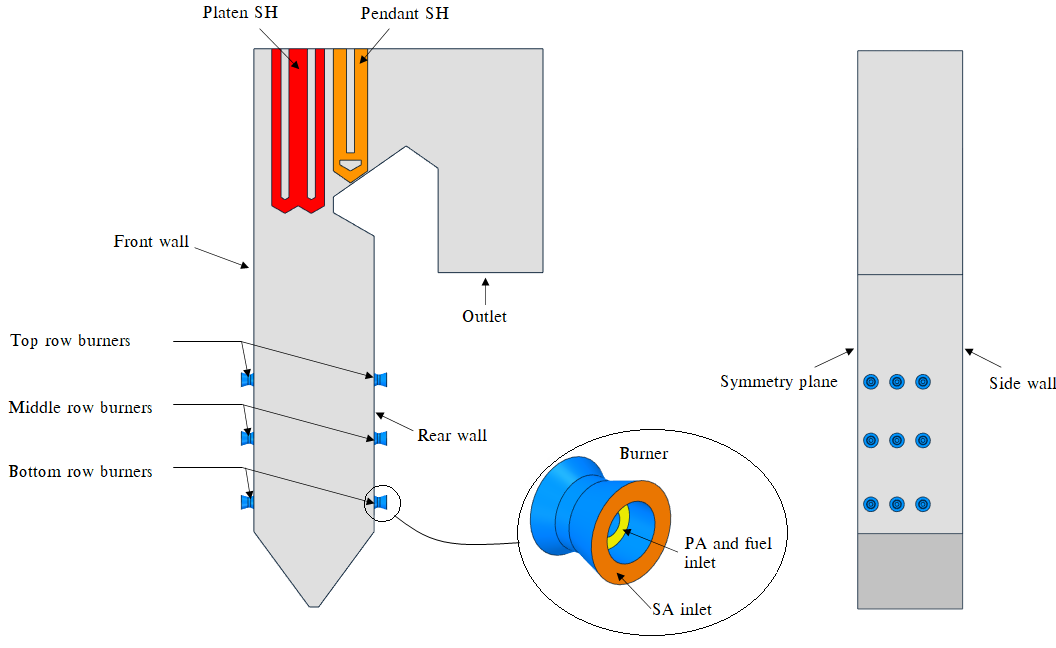
\includegraphics[scale=0.45]{GEOMETRY}}
\caption{Boiler geometry and layout}
\label{fig_geometry}
\end{figure}

The boiler furnace is fed by 6 mills, each supplying a pulverised fuel and primary air (PA) mixture to a burner row consisting of 6 burners. This mixture is injected through the inner burner annulus while the secondary air (SA) is fed through the outer annulus as seen Figure \ref{fig_geometry}. 

The process model of the boiler configuration is shown in Figure \ref{fig_flownex}. The process model includes all the heat exchanging components up till and downstream of the final SH, which include the secondary reheater (RH2), primary SH (SH1), primary reheater (RH1), economiser (EC) and the SA air heaters (SA-AH). The model includes all the relevant attemperators (ATT1, ATT2 and ATT-RH) are inlets and outlets.
\begin{figure}[h!]
\centering
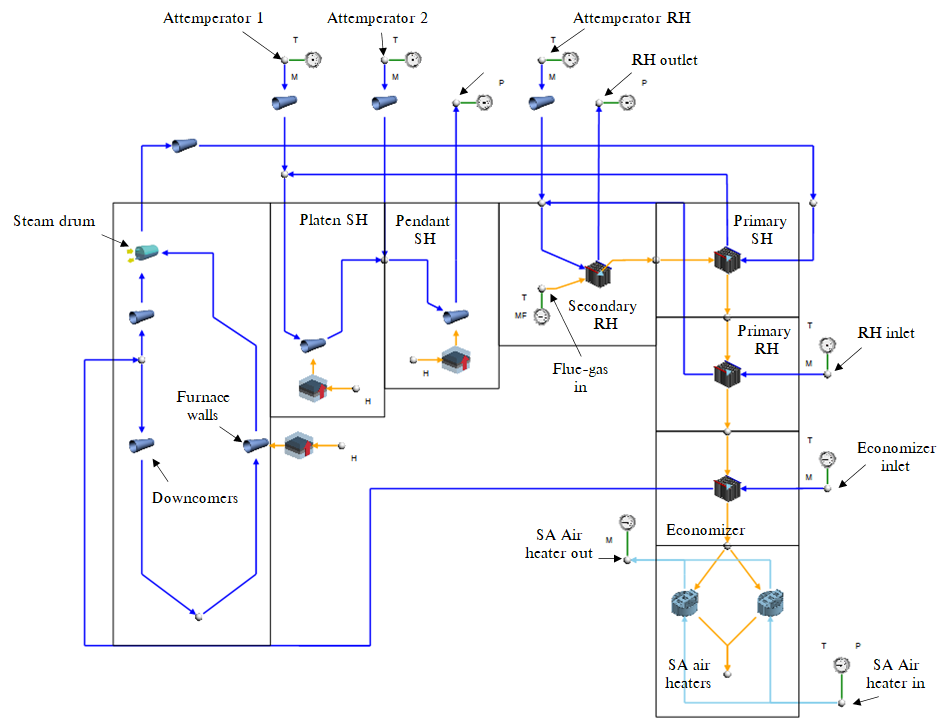
\includegraphics[scale=0.5]{FLOWNEX_SETUP}
\caption{Process model of boiler set-up including the downstream convective components using Flownex SE 2021}
\label{fig_flownex}
\end{figure}

The heat load results of the CFD simulation for the furnace, platen and final SH walls were used as inputs the process model as seen in Figure \ref{fig_flownex}. 
\newpage
\subsection{Model inputs}
Table \ref{tbl_fuel} presents the coal characteristics utilized in the current study along with the coals higher heating value (HHV).\\
\begin{table}[h!]
\centering
\caption{Utility boiler fuel characteristics}
\vspace{5mm}
\label{tbl_fuel}
{\tabulinesep=1.2mm
\begin{tabularx}{\textwidth}{p{0.45\textwidth} p{0.3\textwidth} l}
\hline
\textbf{Fuel constituent} & \textbf{Fraction} & \textbf{Unit}\\
\hline
\textit{Ultimate analysis - (DAF)} & \textit{-} & \textit{-}\\
Carbon & $0.7753$ & $kg/kg_{fuel}$\\
Hydrogen & $0.0415$ & $kg/kg_{fuel}$\\
Nitrogen & $0.0181$ & $kg/kg_{fuel}$\\
Oxygen & $0.1474$ & $kg/kg_{fuel}$\\
Sulphur & $0.0175$ & $kg/kg_{fuel}$\\
\textit{Proximate analysis - (AR)} & \textit{-} & \textit{-}\\
Fixed carbon & $0.340$ & $kg/kg_{fuel}$\\
Volatile matter & $0.196$ & $kg/kg_{fuel}$\\
Ash & $0.4090$ & $kg/kg_{fuel}$\\
Moisture & $0.0550$ & $kg/kg_{fuel}$\\
\hline
\textbf{Energy content - (DAF)} & \textbf{Value} &\\
\hline
Higher heating value & $15070$ & $kJ/kg_{fuel}$\\
\hline
\end{tabularx}}
\end{table}

For a 32\% boiler load the current operational protocol is the to use the bottom front and rear burner rows to meet the low-load demand during start-up.  For this study six cases are simulated in total with the following three burner firing configurations being utilized:
\begin{enumerate}
\item Bottom front and rear row burners are fired (Case 1 \& Case 4)
\item Middle front and rear row burners are fired (Case 2 \& Case 5)
\item Bottom front and middle rear row burners are fired (Case 3 \& Case 6)
\end{enumerate}

Two permutations of the SA flow rate, at the non-firing burners, are used for each of the firing configurations mentioned above. Table \ref{tbl_case_inputs} shows the input conditions for cases 1 to 6. The data is the result of a boilers mass and energy balance calculations.

\begin{table}[h!]
\centering
\caption{Case 1 to 6 model inputs on a per burner basis.}
\label{tbl_case_inputs}
\vspace{5mm}
\label{fuel}
{\tabulinesep=1.2mm
\begin{tabularx}{\textwidth}{p{0.45\textwidth} p{0.25\textwidth} l}
\hline
Active burners & \textbf{Cases 1 - 3} & \textbf{Cases 4 - 6}\\
\hline
\textbf{Fuel flow rate} [$kg/s$]&3.14  &3.14\\
\textbf{PA flow rate} [$kg/s$]&4.95  &4.95\\
\textbf{SA flow rate} [$kg/s$]&14.85  &14.85\\
\hline
Non firing burners &  & \\
\hline
\textbf{SA flow rate} [$kg/s$]&5.0  &2.5\\
\hline
Input air temperatures& &\\
\hline
\textbf{PA} [$K$]&373  &373\\
\textbf{SA} [$K$]&520  &510\\
\hline
\end{tabularx}}
\end{table}

Table \ref{tbl_case_inputs} shows a lower mass flow rate of SA air for case 4 to 6, this was done to compare the expected increase in boiler utilization efficiency, since less dry gas losses are expected, and the effects the drop in the flue-gas mass flow rate has on the convective pass components modelled in the process model. 

\subsection{Numerical solution strategy} 
The CFD simulations were performed using ANSYS Fluent v19.5\textsuperscript{\textregistered} pressure-based solver. the pressure-momentum coupling utilised the SIMPLE technique. Second-order upwinding was used to discretize the momentum, energy and species equations, whereas PRESTO! was used to discretize the pressure equation. The scalar field equations used a second-order upwind scheme.

The spatial discretization for all fields (except pressure) was set to first-order upwind for the first 1000 iterations to ensure a stable solution, after which the discretization order was increased to the above mentioned criteria. For all cases the maximum mass imbalance was 0.024 [$kg/s$] for a total gas flow rate of 190 [$kg/s$] and a heat imbalance of 1770 [$kW$] for a total heat input of 283 [$MW$]. The remaining fields were solved till convergence.

\section{Results \& discussion}
The current section will discuss the results obtained from using the above-mentioned modelling methodologies. The validity of the modelling approach will first be established by comparing the simulation results for MCR load cases (namely 100\%, 80\% and 60\% MCR loads) to that of the experimentally obtained results of the actual plant. Once the model has been shown to demonstrate sufficient accuracy in determining the overall heat loads and combustion characteristics in the boiler furnace at varying loads, the results of the various low-load burner firing configurations are shown and discussed.

\subsection{Model validation}\label{sec_model_valid}
The validation of the proposed model was conducted for three steady-state MCR loads of 100\%, 80\% and 60\%. The model inputs and boundary conditions can be obtained from the study conducted by Laubscher and Rousseau \citep{Laubscher2019b}, where using the same boiler of the present study, they evaluated the thermal performance of the heat exchanging components at full and reduced boiler loads.

\begin{figure}[h!]
	\subfigure[]{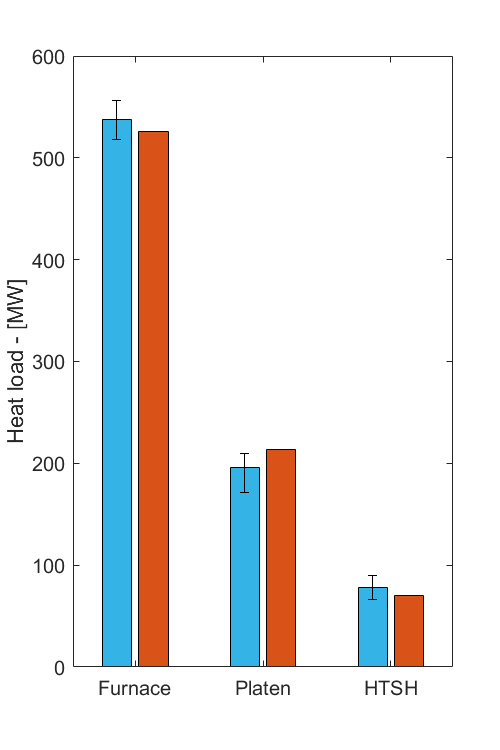
\includegraphics[width=0.32\textwidth]{100_VALID_BAR}}
	\subfigure[]{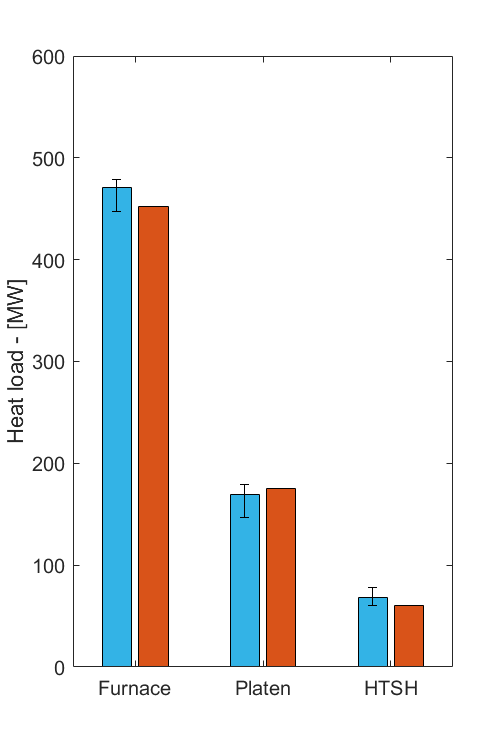
\includegraphics[width=0.32\textwidth]{80_VALID_BAR}}
	\subfigure[]{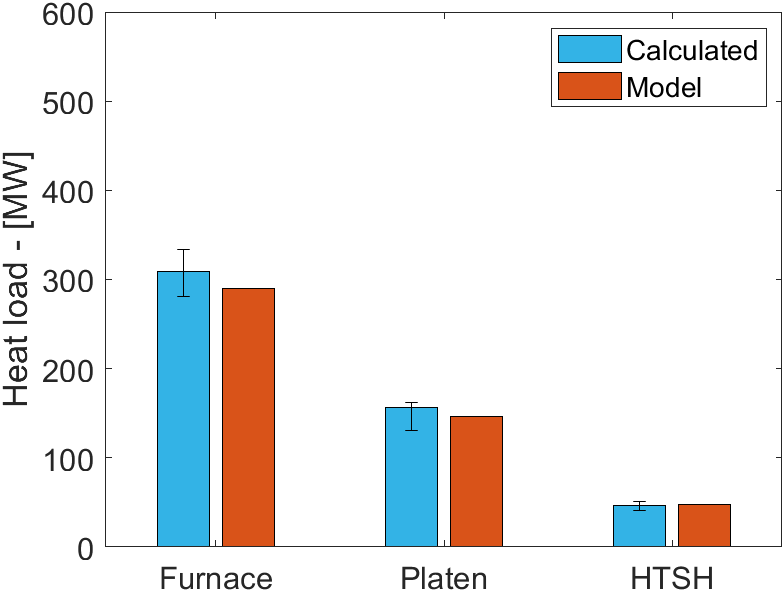
\includegraphics[width=0.32\textwidth]{60_VALID_BAR}}
\caption{Comparison of experimentally calculated and model heat loads for the furnace, platen SH and pendant SH at (a) 100\% MCR, (b) 80\% MCR and (c) 60\% MCR}
\label{fig_heat_valid}
\end{figure}
\clearpage
In Figure \ref{fig_heat_valid} it is shown that the overall heat loads are in good agreement with the calculated results. For the simulated validation loads the proposed model results are within the associated error band, the general trend is an under prediction on the furnace heat loads and an over prediction on the platen super-heater. The pendant super heater illustrate the best comparable results for all load cases.

The CFD model was further validated by comparing the $CO_{ppm}$ and $X_{O_{2}}$ measurements against the CFD results. The probe measurements were taken at a furnace height of 37.5 [$m$] near the center of the boiler during a full load (100\% MCR) operating conditions. The probe is inserted from the side walls to a depth of 4.5 [$m$], measurements were taken every 0.5 [$m$].\\
\begin{figure}[h!]
\centering
\subfigure[]{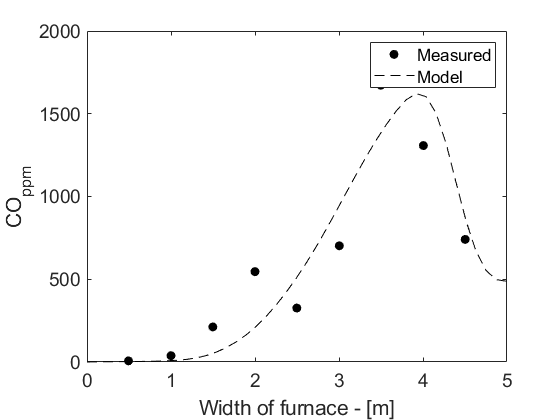
\includegraphics[width = 0.45\textwidth, height =4cm ]{COPPM_VALID}}
\hspace{5mm}
\subfigure[]{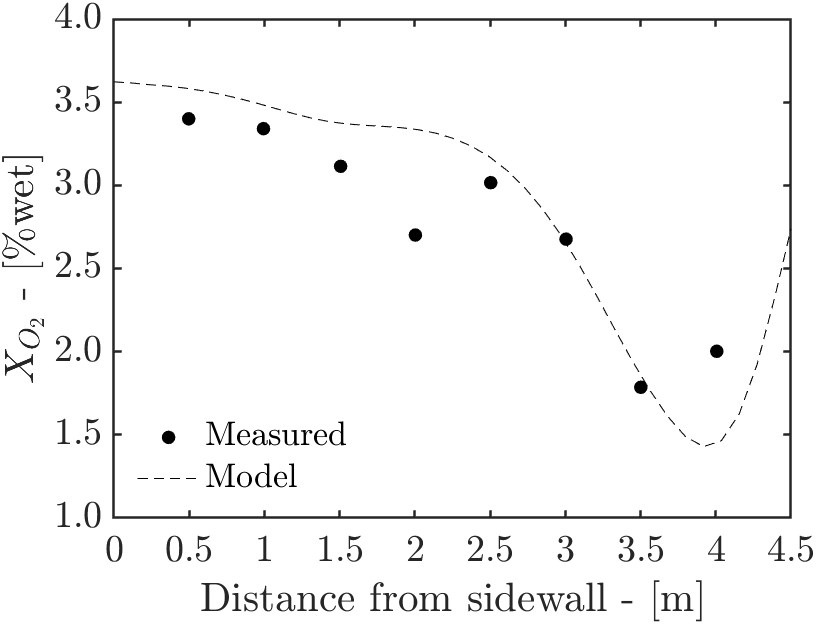
\includegraphics[width = 0.45\textwidth, height =4cm ]{XO2_VALID}}
\caption{Experimentally calculated $CO_{ppm}$ (a) and $X_{O_{2}}$ (b) concentration predictions}
\label{fig_probe_valid}
\end{figure}

Figure \ref{fig_probe_valid} shows the averaged measurement values to that of the CFD predictions. It can be seen that the CFD model can sufficiently resolve the $CO_{ppm}$ and $X_{O_{2}}$ concentrations at the given probe location.
\newpage
\subsection{Simulation results for various burner firing arrangements at 32\% MCR }

Figures \ref{fig_cfd_temp} and \ref{fig_cfd_velo} illustrate the temperature and velocity profiles for the various firing arrangements. With only the middle burner rows firing (Cases 2 and 5) there a is substantial cold region located in the lower half the furnace, resulting in the lowest heat uptake of the furnace for all the cases. This is further exaggerated when considering the Table \ref{tbl_process_parameters} with the mid-firing arrangement producing the lowest steam flow rates resulting in the lowest boiler efficiencies. The bottom firing arrangement (Cases 1 and 4) results in fireball located in the bottom half on the burner, while the mixed firing arrangement (Cases 3 and 6) results is more even distribution of the fireball in the furnace domain. This leads to the highest steam generation rate and boiler efficiency as shown in Table \ref{tbl_process_parameters}.

Figure \ref{fig_cfd_heat_flux} illustrates the heat flux profiles for the simulated cases. Both cases 1 and 4 highlight high heat flux zones near the burner inlets which, in the presence of high temperatures and incomplete combustion near these regions, can lead to high-temperature corrosion \cite{Du2017}. Cases 2 and 5 show that most of the unit heat fluxes are absorbed in the upper half of the boiler, contrary to cases 1 and 4, where the lower half has a higher heat flux absorption, and cases 3 and 6 showing an even distribution throughout the furnace.

The works of Dugum et al \citep{Du2017}, highlights the issue of high-temperature corrosion caused by significant levels of $CO$ ($X_CO$ 0.01 - 0.1) and no-free $O_2$ near regions of high wall temperatures. For low-load operation this phenomena becomes important to avoid since combustion instability can lead to these ideal circumstances. Figure \ref{fig_cfd_coppm} shows the $CO$ molar concentration in the domain located on an iso-surface set 1600 $[K]$. Cases 1 and 4 illustrate the highest likelihood of high-temperature corrosion occurring near the top half of the furnace hopper, furthermore considering Figures \ref{fig_cfd_coppm}(c) and (d) a lower concentration of oxygen is reported.

Investigating the combustion stability for all the cases, symmetry and offset vertical probe plots (as highlighted in Figure \ref{fig_geometry}) are given in Figure \ref{fig_cfd_probe}. The general trends of the $CO_{ppm}$ correspond with each cases burner firing arrangement, as seen with cases 3 and 6, a mixed firing arrangement, where two peaks are observed in the vicinity of the bottom and middle burner rows. Cases 2 and 5 illustrates the highest $X_{O_{2}}$ concentration in the lower half of the burner since there is minimal combustion occurring. The unburnt carbon content and exit flue-gas temperatures for each case are reported in Table \ref{tbl_cfd_results}. With the use of the middle burners (Cases 2 and 5) the highest exit temperature and unburnt carbon content is observed, since the fireball is located in the upper half of the furnace leading to the least possibility of complete combustion due to the shorter residence time. Cases 3 and 6 exhibit the best characteristics with the least amount of unburnt carbon content being observed. It is important to note the effects of a lower SA mass flow rate has on the furnace exit conditions for non-firing burners which generally leads to a hotter exit temperature as is the case with cases 4 to 6. 

The external tube metal temperatures, of Figure \ref{tbl_cfd_results}, were calculated using equation \ref{eqn_t_wall}, which takes into account the temperature drop due to the ash deposit present on platen and final SH.
\begin{equation}\label{eqn_t_wall}
T_{metal} = T_{wall} - \left(\frac{\dot{q}_{SH}t_{ASH}}{\lambda_{ASH}}\right)
\end{equation}
For the platen and final SH the maximum surface temperature are observed for cases 2 and 5. For comparison a 100 \% MCR load the maximum temperatures reported for the platen and final SH are of 500 $[^\circ C]$ and 623 $[^\circ C]$, with the final SH operating in the materials creep range \cite{Laubscher2019b}. Thus, 


Using the process model of Figure \ref{fig_flownex} and the results of the CFD simulations the important process control parameters were determined. 

\begin{figure}\label{fig_cfd_temp}
\centering
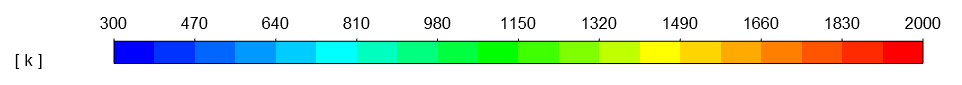
\includegraphics[scale = 0.45]{TEMP_KEY} [$K$]\\
\subfigure[Case 1]{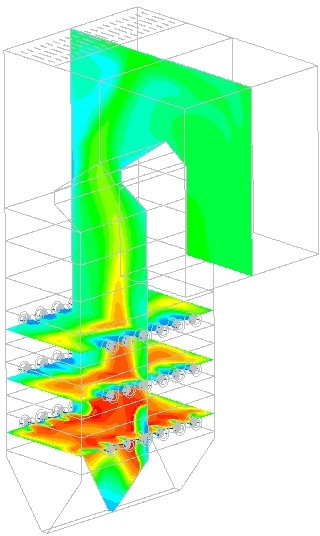
\includegraphics[width=0.32\textwidth]{BOT_TEMP}}
\subfigure[Case 2]{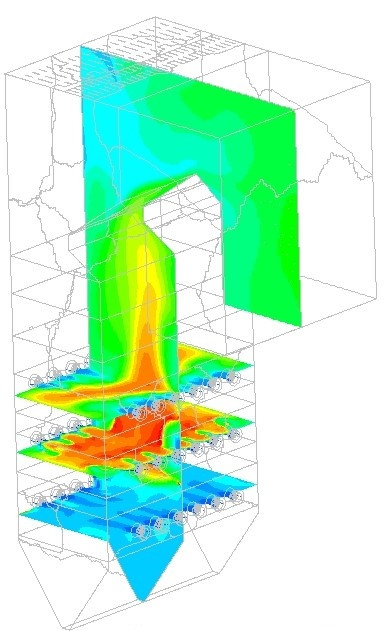
\includegraphics[width=0.32\textwidth]{MID_TEMP}}
\subfigure[Case 3]{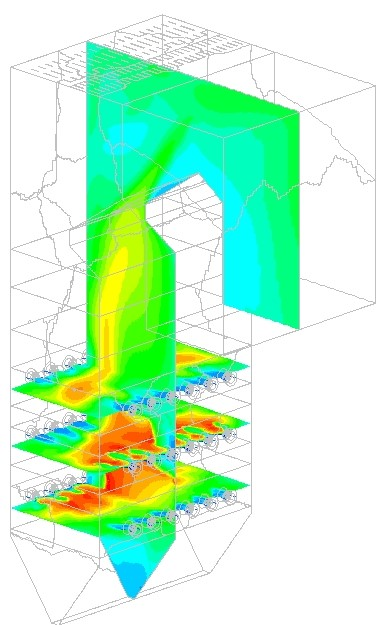
\includegraphics[width=0.32\textwidth]{FBRM_TEMP}}\\
\subfigure[Case 4]{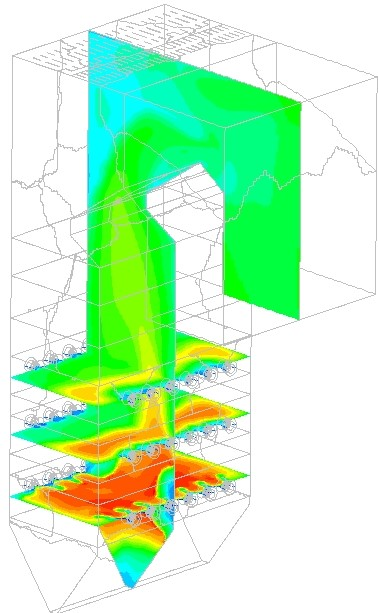
\includegraphics[width=0.32\textwidth]{BOT05_TEMP}}
\subfigure[Case 5]{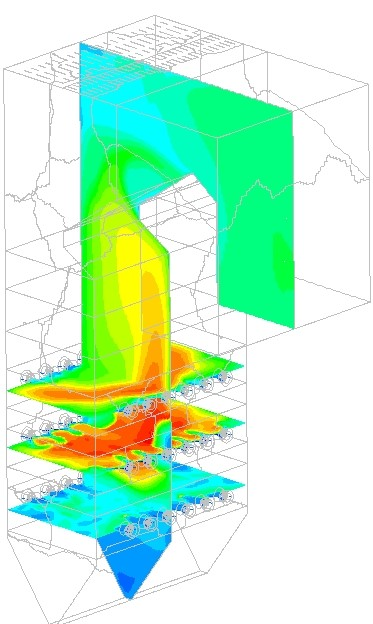
\includegraphics[width=0.32\textwidth]{MID05_TEMP}}
\subfigure[Case 6]{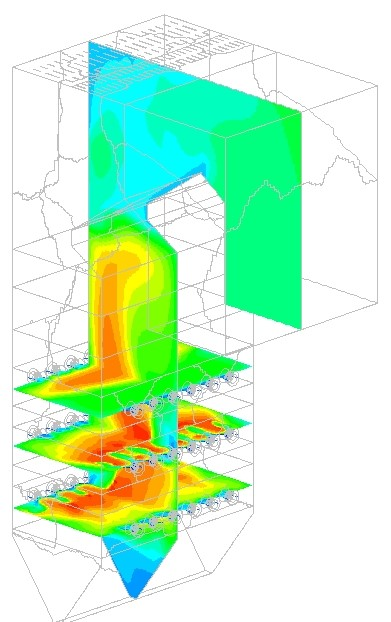
\includegraphics[width=0.32\textwidth]{FBRM05_TEMP}}
\caption{Temperature fields for cases 1 through 6 [(a)-(f)]}
\end{figure}


\begin{figure}[h!]\label{fig_cfd_velo}
\centering
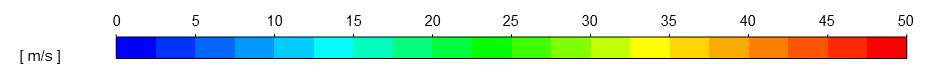
\includegraphics[scale = 0.45]{VEL_KEY} [$m/s$]\\
\subfigure[Case 1]{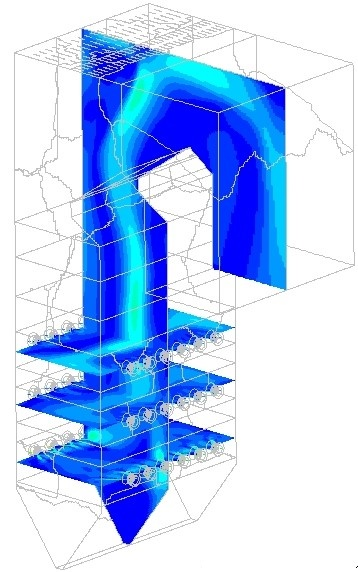
\includegraphics[width=0.32\textwidth]{BOT_VEL}}
\subfigure[Case 2]{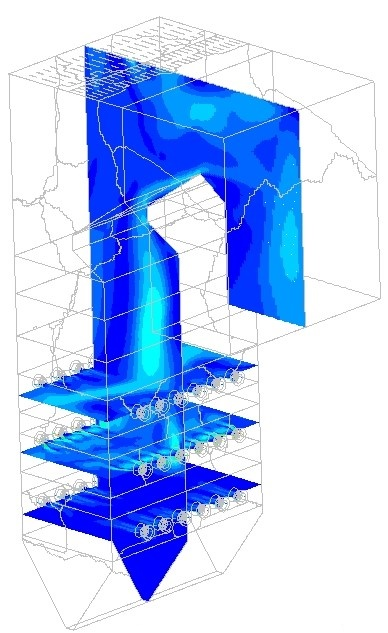
\includegraphics[width=0.32\textwidth]{MID_VEL}}
\subfigure[Case 3]{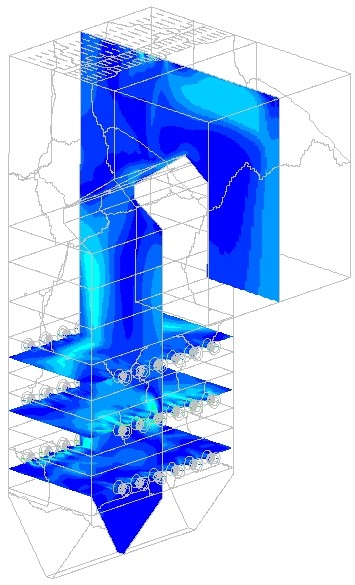
\includegraphics[width=0.32\textwidth]{FBRM_VEL}}\\
\subfigure[Case 4]{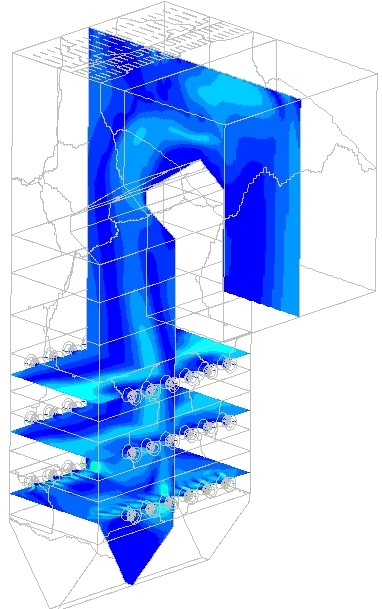
\includegraphics[width=0.32\textwidth]{BOT05_VEL}}
\subfigure[Case 5]{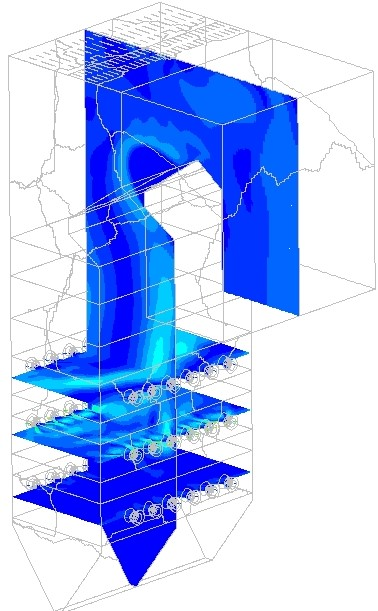
\includegraphics[width=0.32\textwidth]{MID05_VEL}}
\subfigure[Case 6]{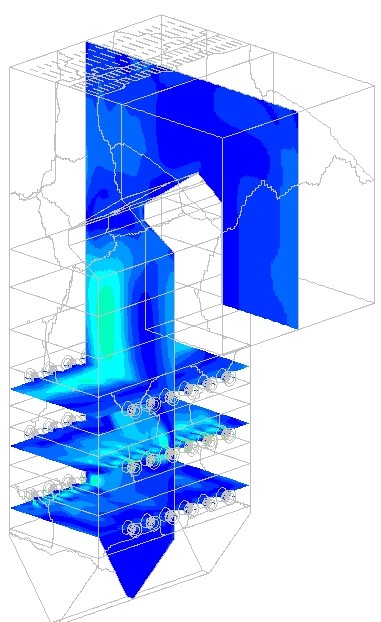
\includegraphics[width=0.32\textwidth]{FBRM05_VEL}}
\caption{Velocity fields for cases 1 through 6 [(a)-(f)]}
\end{figure}

\begin{figure}[h!]\label{fig_cfd_heat_flux}
\centering
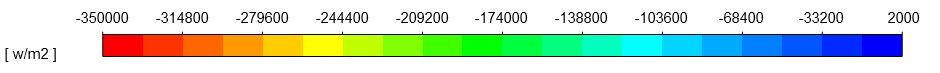
\includegraphics[scale = 0.45]{HEATFLUX_KEY} [$W/m^2$]\\
\subfigure[Case 1]{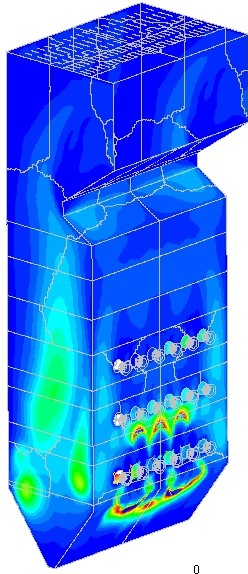
\includegraphics[scale = 0.29]{BOT_HEATFLUX}}
\hspace{5mm}
\subfigure[Case 2]{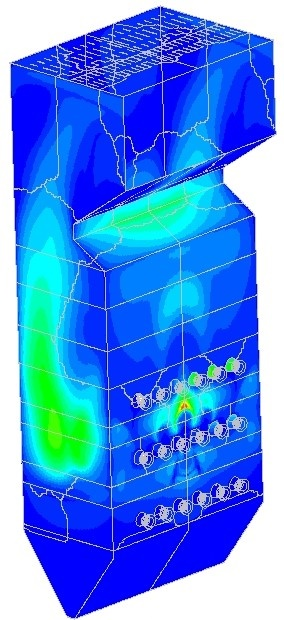
\includegraphics[scale = 0.35]{MID_HEATFLUX}}
\hspace{5mm}
\subfigure[Case 3]{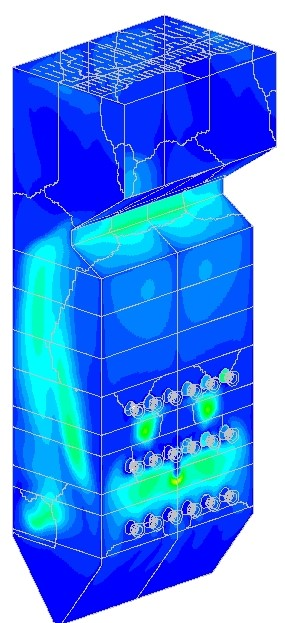
\includegraphics[scale = 0.35]{FBRM_HEATFLUX}}\\
\subfigure[Case 4]{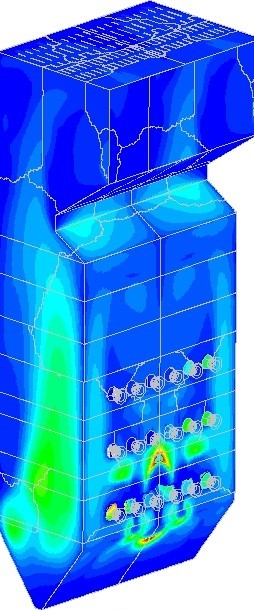
\includegraphics[scale = 0.35]{BOT05_HEATFLUX}}
\hspace{5mm}
\subfigure[Case 5]{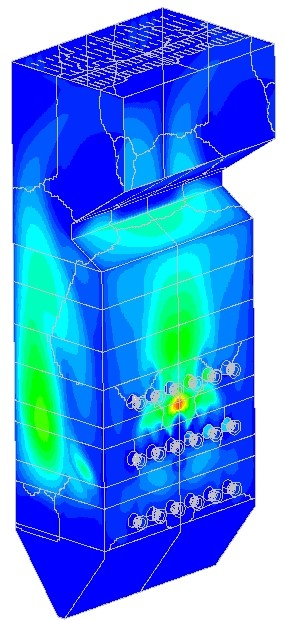
\includegraphics[scale = 0.35]{MID05_HEATFLUX}}
\hspace{5mm}
\subfigure[Case 6]{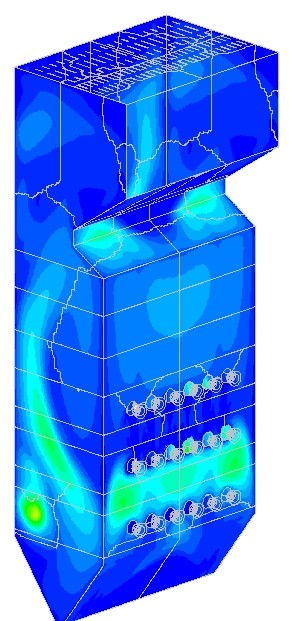
\includegraphics[scale = 0.35]{FBRM05_HEATFLUX}}
\caption{Heat fluxes profiles for cases 1 through 6 [(a)-(f)]}
\end{figure}

\begin{figure}\label{fig_cfd_coppm}
\centering
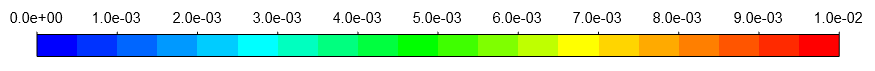
\includegraphics[scale=0.45]{CO_MF_KEY} [$X_{CO}$] \\
\subfigure[Case 1]{	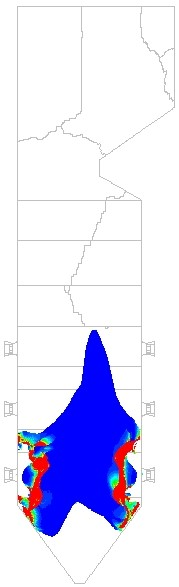
\includegraphics[width=0.18\textwidth, height = 7cm]{BOT_ISO_COPPM_F}
				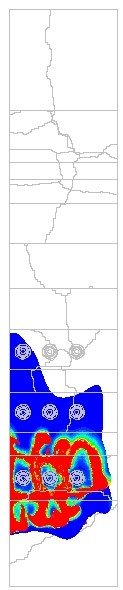
\includegraphics[height = 7cm]{BOT_ISO_COPPM_S}}
\subfigure[Case 2]{	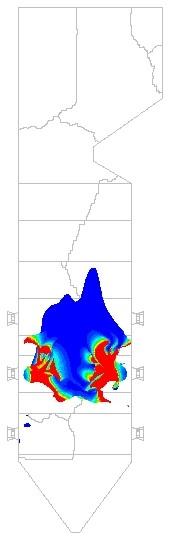
\includegraphics[width=0.18\textwidth, height = 7cm]{MID_ISO_COPPM_F}
				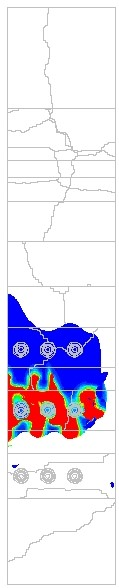
\includegraphics[height = 7cm]{MID_ISO_COPPM_S}}
\subfigure[Case 3]{	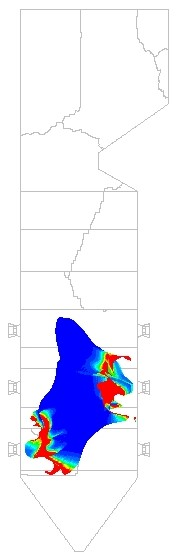
\includegraphics[width=0.18\textwidth, height = 7cm]{FBRM_ISO_COPPM_F}
				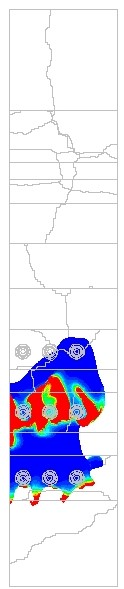
\includegraphics[height = 7cm]{FBRM_ISO_COPPM_S}}\\
\subfigure[Case 4]{	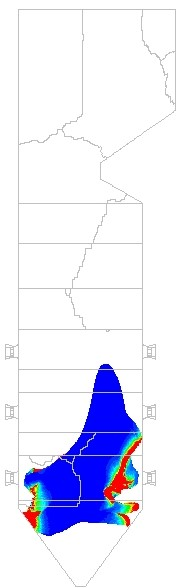
\includegraphics[width=0.18\textwidth, height = 7cm]{BOT05_ISO_COPPM_F}
				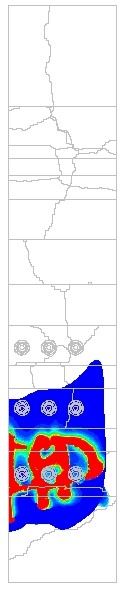
\includegraphics[height = 7cm]{BOT05_ISO_COPPM_S}}
\subfigure[Case 5]{	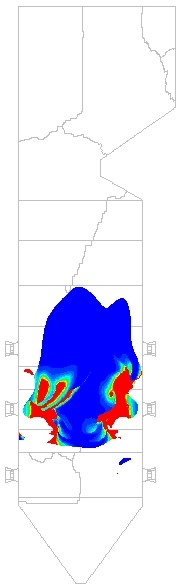
\includegraphics[width=0.18\textwidth, height = 7cm]{MID05_ISO_COPPM_F}
				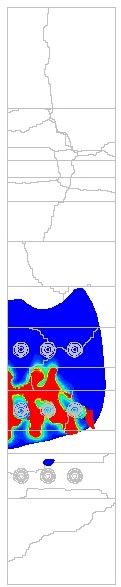
\includegraphics[height = 7cm]{MID05_ISO_COPPM_S}}
\subfigure[Case 6]{	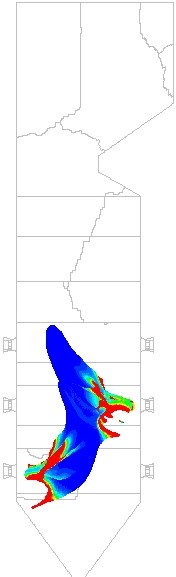
\includegraphics[width=0.18\textwidth, height = 7cm]{FBRM05_ISO_COPPM_F}
				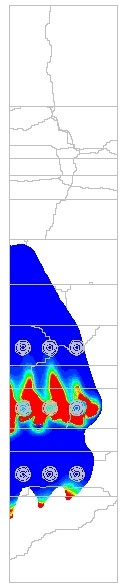
\includegraphics[height = 7cm]{FBRM05_ISO_COPPM_S}}\\
\caption{CO molar fraction ($X_{CO}$) concentrations for cases 1 through 6 [(a)-(f)] on a temperature iso-surface of 1600 K}
\end{figure}


\begin{figure}[h!]\label{fig_cfd_probe}
\centering
\subfigure[Symmetry vertical plot]{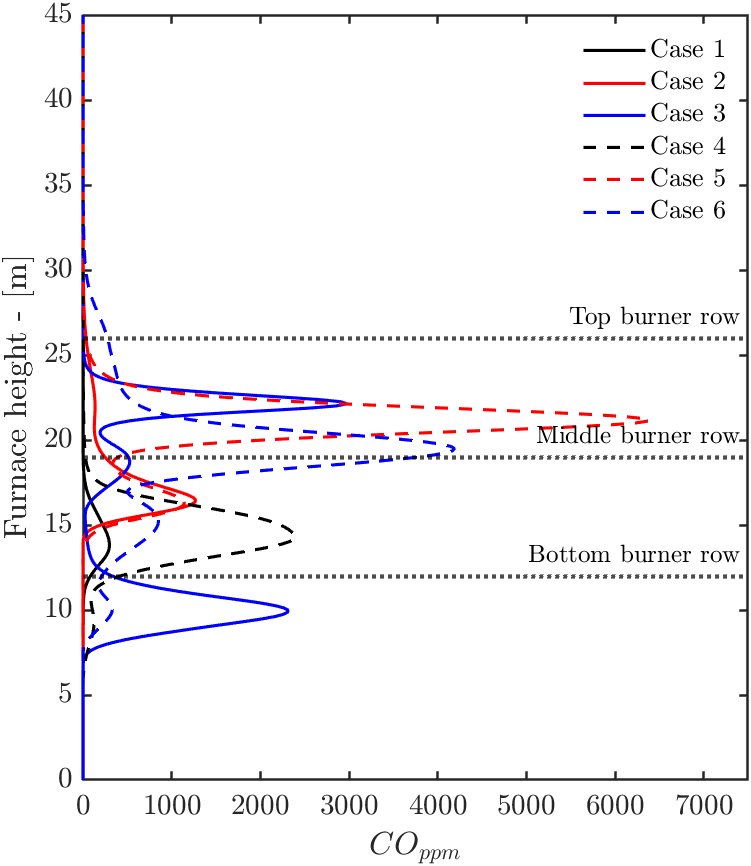
\includegraphics[scale = 0.36]{SYMMETRY_PROBE_COPPM}}
\hspace{5mm}
\subfigure[Offset vertical plot]{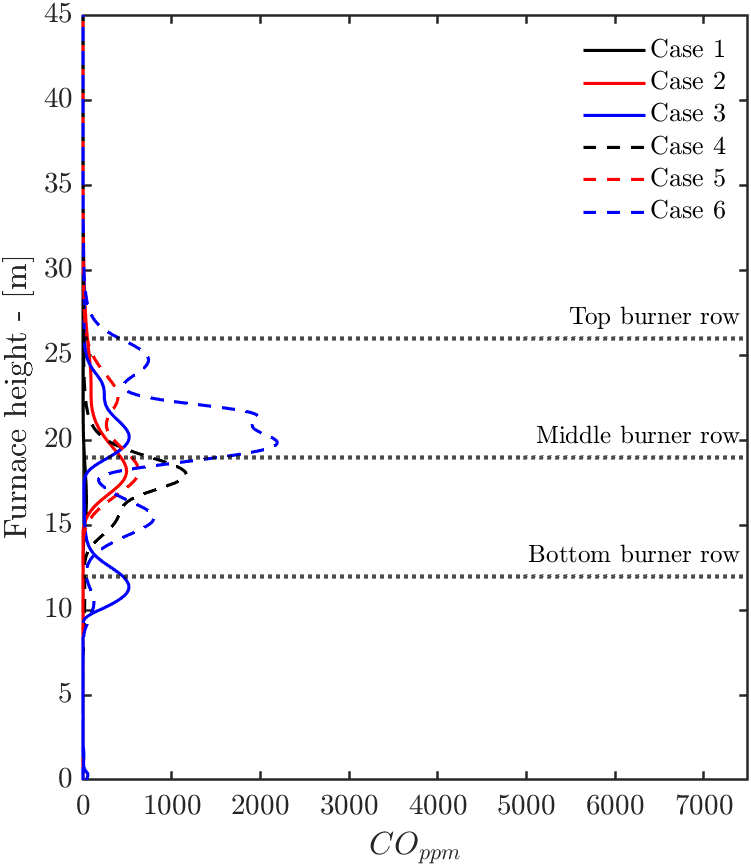
\includegraphics[scale = 0.36]{OFFSET_PROBE_COPPM}}\\
\subfigure[Symmetry vertical plot]{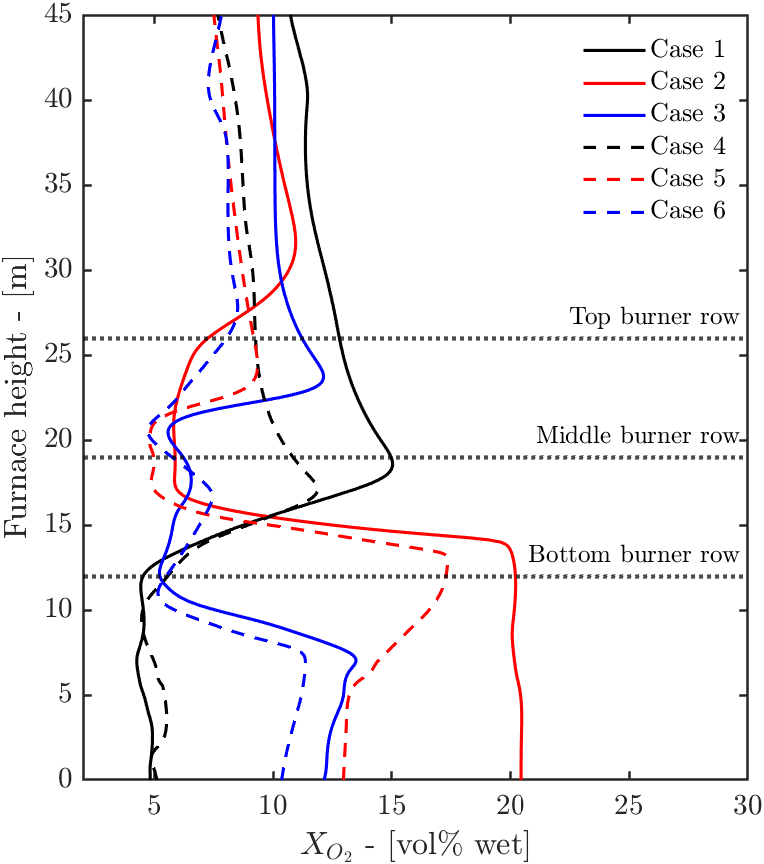
\includegraphics[scale = 0.35]{SYMMETRY_PROBE_XO2}}
\hspace{5mm}
\subfigure[Offset vertical plot]{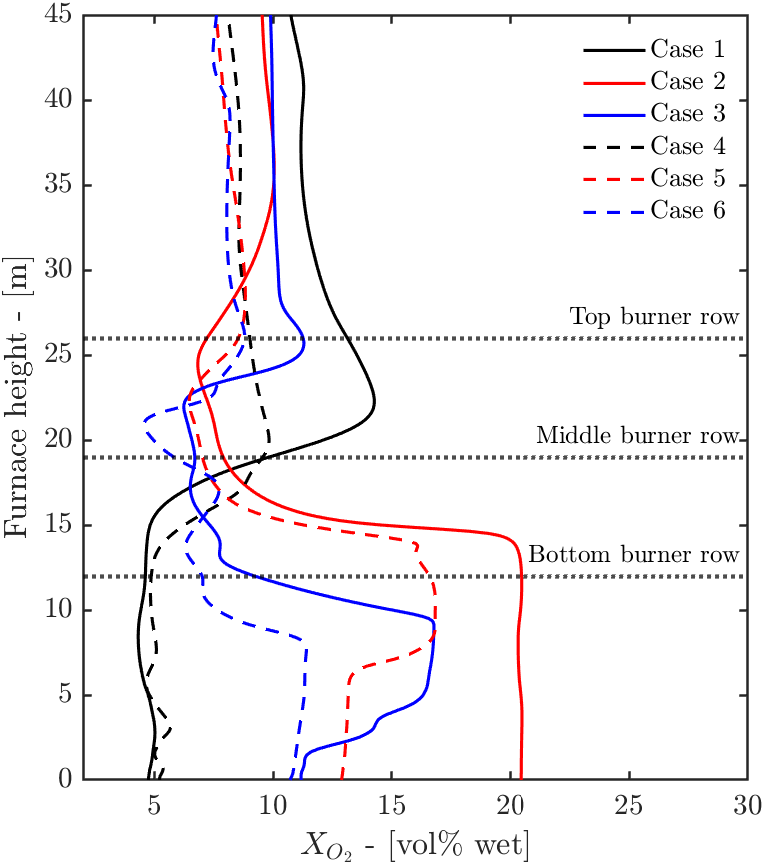
\includegraphics[scale = 0.35]{OFFSET_PROBE_XO2}}

\caption{$CO_{PPM}$ [(a) and (b)] and $X_{O_{2}}$ [(c) and (d)] line plots on symmetry and offset vertical probe lines}
\end{figure}



\begin{table}[h!]\label{tbl_process_parameters}
\centering
\caption{Process model control parameters}
\label{fuel}
{\tabulinesep=1.2mm
\begin{tabularx}{\linewidth}{p{0.45\linewidth} XXXXXX}
\hline
&\multicolumn{6}{c}{Cases}\\
 & \textbf{1} & \textbf{2} & \textbf{3}& \textbf{4}&\textbf{5}&\textbf{6}\\
\hline
\textbf{Main steam flow rate} 	[$kg/s$]		&175.8&172.9&180.5&180.2&179.1&184.1 \\
\textbf{Main steam exit temp} 	[$^{\circ}C$]	&535& 535 &535&535 &535& 535\\
\textbf{RH steam flow rate} 	[$kg/s$]		&158.2&155.6&162.5&162.2&161.2&165.6\\
\textbf{RH steam exit temp} 	[$^{\circ}C$]	&524&527&531&520&510&512\\
\textbf{Boiler efficiency} 		[$\%$]			&85.3&84.1&87.9	&87.2&85.9&89.1\\
\textbf{ATT1} 		[$kg/s$]					&10.4&16.9&13.9&7.9&5.5&10.9\\
\textbf{ATT2} 		[$kg/s$]					&1.7&3.8&4.2&3.8&3.67&4.2\\
\textbf{ATT-RH} 		[$kg/s$]				&0.0&0.0&0.0&0.0&0.0&0.0\\
\hline
\end{tabularx}}
\end{table}

\begin{table}[h!]\label{tbl_cfd_results}
\centering
\caption{Furnace exit conditions and SH wall temperatures}
\label{fuel}
{\tabulinesep=1.2mm
\begin{tabularx}{\linewidth}{p{0.4\linewidth} XXXXXX}
\hline
&\multicolumn{6}{c}{Cases}\\
 & \textbf{1} & \textbf{2} & \textbf{3}& \textbf{4}&\textbf{5}&\textbf{6}\\
\hline
\multicolumn{7}{l}{\textit{Furnace exit}}\\
\textbf{Exit temperature} [$K$] & 1168 & 1230 & 1215 & 1208 & 1306 & 1298\\
\textbf{Unburnt carbon} [$(\times 10^{-3})\,\%$] & 1.83 & 1.94 & 1.54 & 1.81 & 1.89 & 1.62\\
\multicolumn{7}{l}{\textit{Platen SH}}\\
\textbf{Max wall temperature} [$^{\circ}C$]  &477 & 492 & 481  & 480 & 493 & 490\\
\textbf{Mean wall temperature} [$^{\circ}C$] &439 & 453 & 446 & 454 & 442 & 451\\
\multicolumn{7}{l}{\textit{Final SH}}\\
\textbf{Max wall temperature} [$^{\circ}C$]  & 602 & 624 & 608 & 595 & 626 & 612\\
\textbf{Mean wall temperature} [$^{\circ}C$] & 520 & 523 & 517 & 512 & 520 & 511\\
\hline
\end{tabularx}}
\end{table}


\begin{table}[h!]
\centering
\caption{Radiative heat transfer percentage for the platen and pendant SH}
\label{fuel}
{\tabulinesep=1.2mm
\begin{tabularx}{\linewidth}{p{0.25\linewidth} XX}
\hline
&\multicolumn{2}{c}{Cases}\\
 &\textbf{3}&\textbf{6}\\
\hline
Evaporator \\
Platen SH [\%] & \\
Pendant SH [\%] &\\
Secondary RH [\%]\\
Primary SH [\%]\\
Primary RH [\%]\\
Economiser [\%]\\
\hline
\end{tabularx}}
\end{table}

\clearpage
\section{Conclusions}
ghhhb
jyjjf
\section*{Acknowledgements}
The authors would like to thank the Eskom EPPEI program for financially supporting the present study and acknowledge the computational resources provided by the Centre for High Performance Computing (CHPC), South Africa.

\section*{References}

\bibliography{PAPER1_LOW_LOAD}

\end{document}
